\section{Účelová funkce}

Cílem zbytku navržené neuronové sítě je z časoprostorových příznaků získaných v předchozích částech vytvořit výslednou hustotní mapu.
Specificky má síť za úkol vytvořit hustotní mapu, která odpovídá "základní pravdě" (Ground Truth), posledního snímku právě zpracovávané sekvence vstupních snímků.
Jednou z možností by bylo učit síť co nejblíže replikovat hustotní mapy tvořené Gaussiány vložené do hustotní mapy v bodech, kde se v posledním snímku nacházejí jednotlivé lidské hlavy, jak bylo popsáno v kapitole \ref{sec:History}.
V takovémto případě je často použita účelová funkce, které je definovaná na základě sumy chyby v jednotlivých bodech výsledného obrazu. Příkladem by mohla být například střední kvadratická chyba \ref{eq:MSE_loss}, nebo nebo absolutní chyba \ref{eq:AE_loss}.

\begin{equation}
loss_{MSE} = \frac{1}{n} \sum_{i=1}^{n} (x_i - y_i)^2
\label{eq:MSE_loss}
\end{equation}

\begin{equation}
loss_{AE} = \frac{1}{n} \sum_{i=1}^{n} |x_i - y_i|
\label{eq:AE_loss}
\end{equation}

Dle \cite{Bayesian_Crowd_Counting, DM_Count} ale není využití těchto účelových funkcí závislých na jednotlivých pixelech optimální, jelikož výsledná přesnost natrénované neuronové sítě je silně závislá na kvalitě vygenerovaných hustotních map základní pravdy.
Získání vysoce kvalitní základní pravdy je ale obtížné.
Datasety používané pro trénování neuronových sítí jsou totiž velmi obsáhlé a manuální anotace jednotlivých snímků, kde musí být označena každá hlava je proto časově velmi náročné.
Anotace se z toho důvodu u mnoha významných datasetů omezuje pouze na pozice hlav a nijak nebere v potaz jejich velikost v obraze. U Gaussiánů je proto často použit konstantní parametr rozptylu a vliv perspektivy způsobující rozdílné velikosti hlav v obraze není nijak brán v úvahu.
Problémem může být také přesné určení pozice hlavy, kvůli částečným zakrytím, ke kterým může v obraze docházet.
Jednotliví lidé anotující datasety také mohou mít jiné preference k tomu, kam bod označující hlavu umisťují. V některých případech to může například být doprostřed čela, jindy ale třeba na nos.
Tyto faktory znamenají, že vygenerovaná hustotní mapa často není optimální, což může vést ke zhoršení přesnosti trénované sítě.

Z tohoto důvodu byla v navržené síti použita účelová funkce navržená ve článku Distribution Matching for Crowd Counting \cite{DM_Count}.
Metoda navržená v tomto článku se na problém počítání objektů v obraze dívá jako na problém párování distribučních funkcí (Distribution Matching) a jejím výstupem je hustotní mapa, pro kterou platí, že suma jejích jednotlivých bodů se rovná počtu lidí v obraze, stejně jako u metody vkládající do mapy Gaussiány. Narozdíl od této metody ale Gaussiány nepotřebuje.

Tato účelová funkce se skládá ze tří částí.
Tyto tři části jsou menšími účelovými funkcemi, které jsou ve výsledné funkci spojeny dohromady pomocí lineární kombinace.
První z nich autoři nazývají "Counting Loss".
Ta je definovaná vzorcem \ref{eq:counting_loss}.
Základní pravda je v následujících vzorcích vyjádřena písmenem \(z\), které reprezentuje binární mapu pozic jednotlivých hlav v obraze, zatímco \(\hat{z}\) reprezentuje predikovanou hustotní mapu.
\(\|z\|_1\) a \(\|\hat{z}\|_1\) jsou L1 normami vektorizovaných matic \(z\) a \(\hat{z}\) a vyjadřují počet lidí v základní pravdě a v predikované hustotní mapě.
Counting loss je vyjádřena jako absolutní hodnota rozdílu těchto počtů a jejím cílem je při hledání optima konečné účelové funkce zajistit, aby se predikovaný počet co nejvíce blížil opravdovému počtu lidí v obraze.

\begin{equation}
loss_C(z, \hat{z}) = \Big|\|{z}\|_1 - \|\hat{z}\|_1\Big|
\label{eq:counting_loss}
\end{equation}

Druhou částí účelové funkce je tzv. "Optimal Transport Loss". 
Tato funkce využívá metod z matematické oblasti dopravních problémů.
Jedním z prvních matematiků, který se touto oblastí zabýval byl Gaspard Monge, vévoda z Péluse, který se v roce 1781 zabýval problematikou konstrukce vojenského opevnění a tvorbu takové stavby zefektivnit.
Přesněji se zaměřil na konstrukci příkopů a valů.
Je logické, že při konstrukci valu chceme využít zeminu, která byla vykopána z příkopu.
Všechna tato zemina ale musí být přesunuta, a z ekonomických důvodů chceme, aby k přesunu došlo co nejoptimálnějším způsobem.
Práce vynaložená na přesun zeminy z příkopu na val tedy musí být co nejnižší.

\begin{figure}[h!]
	\centering
	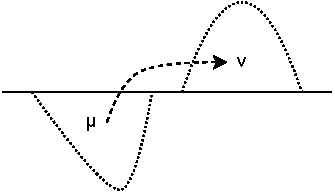
\includegraphics[width=0.5\textwidth]{Figures/solution/Optimal_transport.pdf}
	\caption{Ukázka problému optimálního přesunu}
	\label{fig:RNN_architecture}
\end{figure}


Příkop, ze kterého je zemina brána je označen písmenem \(\mu\) a val, na který je vršena písmenem \(\nu\).
Je jasné, že hmota při přemisťování nemůže vznikat ani zanikat, takže objem hmoty navršené na val musí být roven objemu hmoty vykopané z příkopu. 
Rozložení \(\mu\) a \(\nu\) tedy můžeme vyjádřit jako pravděpodobnostní míry na prostorech \(X\) a \(Y\).
Dále můžeme definovat funkci ceny \(c : X \times Y  \rightarrow \R^+ \), která vyjadřuje práci nutnou k přemístění jedné jednotky hmoty z bodu \(x \in X\) do bodu \(y \in Y\).
Mongeho-Kantorovichův problém optimálního přesunu (Optimal Transport) se zabývá tím, jak přesunout všechnu hmotu z \(\mu\) do \(\nu\) tak, aby celková cena přesunu \(c\) byla minimální.

V \cite{DM_Count} definují optimální přesun pomocí vzorce \ref{eq:ot_1}, kde \(C\) značí matici obsahující všechny ceny přemístění bodu z \(\mu\) a \(\nu\) a \(\Gamma\) je množinou všech možných způsobů, jak tyto body přemístit.

\begin{equation}
\mathcal{W}(\mu, \nu) = \min_{\gamma in \Gamma} \langle C, \gamma \rangle
\label{eq:ot_1}
\end{equation}

Tato minimální cena může být použita jako metrika pro porovnání podobnosti dvou měr pravděpodobnosti.
Můžeme na to dívat tak, že čím méně zeminy musí být přemístěno z hromady \(\mu\), abychom dostali hromadu \(\nu\), tím podobnější si \(\mu\) a \(\nu\) musí být.
Optimal Transport Loss přesně tohoto principu využívá pro porovnání výsledné predikce sítě a 
základní pravdy.
Aby se tyto mapy daly pomocí Mongeho-Kantorovichova optimálního přesunu porovnat, jsou před výpočtem metriky znormalizovány, aby suma přes obě z nich byla rovna jedné.
Jako cenovou funkci použili autoři \cite{DM_Count} kvadrát Euklidovské vzdálenosti bodů v planární mapě \(c(z(i), \hat{z}(j)) = \|z(i) - \hat{z}(j)\|_2^2\), kde \(z(i)\) a \(\hat{z}(j)\) jsou koordináty bodů \(i\) a \(j\).

\begin{equation}
loss_{OT}(z, \hat{z}) = \mathcal{W}\bigg(\frac{z}{\|z\|_1}, \frac{\hat{z}}{\|\hat{z}\|_1}\bigg) 
\label{eq:ot_loss}
\end{equation}

Pro získání gradientu, který může být sítí zpětně šířen a na jehož základě dojde k přenastavení jejích vah, použili autoři duální problém k optimálnímu přesunu, jenž byl formulován Leonidem Kantorovičem.
Caffarelli \cite{Caffarelli_dual_problem} tento problém připodobňuje k situaci, kdy je pro přemístění zeminy z \(\mu\) do \(\nu\) použit externí přepravce, který si v nechává platit v bodě naložení \(\mu(x_i)\) a v bodě vyložení \(\nu(x_i)\).
Jeho ceny nesmí být vyšší, než cena \(c(x_i, y_i)\), jelikož to by bylo pro objednatele přepravy nevýhodné a přepravce by si proto neobjednal.
Přepravce proto řeší, jak nastavit ceny, aby maximalizoval svůj zisk, avšak jeho cena nebyla vyšší, než cena, kterou by platil objednavatel, kdyby převoz zeminy organizoval sám.
V \cite{DM_Count} je tento problém formulován rovnicí \ref{eq:ot_2}, kde \(\alpha\) a \(\beta\) jsou výplatní funkce, udávající, kolik si přepravce účtuje za naložení a vyložení materiálu.

\begin{equation}
\mathcal{W}(\mu, \nu) = \max_{\alpha, \beta \in \R^n} \langle \alpha, \mu \rangle + \langle \beta, \nu \rangle; \alpha_i + \beta_j  \leq c(x_i, y_j),  \forall i, j
\label{eq:ot_2}
\end{equation}

Rovnice \ref{eq:ot_loss} lze s použitím duálního problému přepsat jako \( loss_{OT}(z, \hat{z}) = \bigg \langle \alpha^*, \frac{z}{\|z\|_1} \bigg \rangle + \bigg \langle \beta^*, \frac{\hat{z}}{\|\hat{z}\|_1} \bigg \rangle \), kde  \(\alpha^*\) a \(\beta^*\) jsou řešeními \ref{eq:ot_2}, z čehož se dá vypočítat gradient.

\begin{equation}
\frac{\partial loss_{OT}}{\partial \hat{z}} = \frac{\beta^*}{\|\hat{z}\|_1} - \frac{ \langle \beta^*, \hat{z} \rangle}{\|\hat{z}\|_1^2}
\label{eq:ot_2}
\end{equation}

Pro zjištění řešení \(\alpha^*\) a \(\beta^*\) používají autoři Sinkhornův algoritmus.
Při jeho použití síť z počátku rychle konverguje do lokálního optima, avšak tato konvergence se také rychle zpomaluje.
Dle autorů toto zpomalování způsobí, že jelikož je trénování sítě po určitém počtu trénovacích epoch ukončeno, síť nikdy optima nedosáhne.
Predikovaná hustotní mapa proto bude velice podobná základní pravdě, ale nebude identická.
Problémy podle autorů nastávají hlavně v těch částech scény, kde je hustota lidí nízká a lidé jsou separovaní.

\begin{figure}[h!]
	\centering
	% GNUPLOT: LaTeX picture with Postscript
\begingroup
  \makeatletter
  \providecommand\color[2][]{%
    \GenericError{(gnuplot) \space\space\space\@spaces}{%
      Package color not loaded in conjunction with
      terminal option `colourtext'%
    }{See the gnuplot documentation for explanation.%
    }{Either use 'blacktext' in gnuplot or load the package
      color.sty in LaTeX.}%
    \renewcommand\color[2][]{}%
  }%
  \providecommand\includegraphics[2][]{%
    \GenericError{(gnuplot) \space\space\space\@spaces}{%
      Package graphicx or graphics not loaded%
    }{See the gnuplot documentation for explanation.%
    }{The gnuplot epslatex terminal needs graphicx.sty or graphics.sty.}%
    \renewcommand\includegraphics[2][]{}%
  }%
  \providecommand\rotatebox[2]{#2}%
  \@ifundefined{ifGPcolor}{%
    \newif\ifGPcolor
    \GPcolortrue
  }{}%
  \@ifundefined{ifGPblacktext}{%
    \newif\ifGPblacktext
    \GPblacktexttrue
  }{}%
  % define a \g@addto@macro without @ in the name:
  \let\gplgaddtomacro\g@addto@macro
  % define empty templates for all commands taking text:
  \gdef\gplbacktext{}%
  \gdef\gplfronttext{}%
  \makeatother
  \ifGPblacktext
    % no textcolor at all
    \def\colorrgb#1{}%
    \def\colorgray#1{}%
  \else
    % gray or color?
    \ifGPcolor
      \def\colorrgb#1{\color[rgb]{#1}}%
      \def\colorgray#1{\color[gray]{#1}}%
      \expandafter\def\csname LTw\endcsname{\color{white}}%
      \expandafter\def\csname LTb\endcsname{\color{black}}%
      \expandafter\def\csname LTa\endcsname{\color{black}}%
      \expandafter\def\csname LT0\endcsname{\color[rgb]{1,0,0}}%
      \expandafter\def\csname LT1\endcsname{\color[rgb]{0,1,0}}%
      \expandafter\def\csname LT2\endcsname{\color[rgb]{0,0,1}}%
      \expandafter\def\csname LT3\endcsname{\color[rgb]{1,0,1}}%
      \expandafter\def\csname LT4\endcsname{\color[rgb]{0,1,1}}%
      \expandafter\def\csname LT5\endcsname{\color[rgb]{1,1,0}}%
      \expandafter\def\csname LT6\endcsname{\color[rgb]{0,0,0}}%
      \expandafter\def\csname LT7\endcsname{\color[rgb]{1,0.3,0}}%
      \expandafter\def\csname LT8\endcsname{\color[rgb]{0.5,0.5,0.5}}%
    \else
      % gray
      \def\colorrgb#1{\color{black}}%
      \def\colorgray#1{\color[gray]{#1}}%
      \expandafter\def\csname LTw\endcsname{\color{white}}%
      \expandafter\def\csname LTb\endcsname{\color{black}}%
      \expandafter\def\csname LTa\endcsname{\color{black}}%
      \expandafter\def\csname LT0\endcsname{\color{black}}%
      \expandafter\def\csname LT1\endcsname{\color{black}}%
      \expandafter\def\csname LT2\endcsname{\color{black}}%
      \expandafter\def\csname LT3\endcsname{\color{black}}%
      \expandafter\def\csname LT4\endcsname{\color{black}}%
      \expandafter\def\csname LT5\endcsname{\color{black}}%
      \expandafter\def\csname LT6\endcsname{\color{black}}%
      \expandafter\def\csname LT7\endcsname{\color{black}}%
      \expandafter\def\csname LT8\endcsname{\color{black}}%
    \fi
  \fi
    \setlength{\unitlength}{0.0500bp}%
    \ifx\gptboxheight\undefined%
      \newlength{\gptboxheight}%
      \newlength{\gptboxwidth}%
      \newsavebox{\gptboxtext}%
    \fi%
    \setlength{\fboxrule}{0.5pt}%
    \setlength{\fboxsep}{1pt}%
\begin{picture}(7200.00,4320.00)%
    \gplgaddtomacro\gplbacktext{%
      \colorrgb{0.00,0.00,0.00}%%
      \put(708,652){\makebox(0,0)[r]{\strut{}$0$}}%
      \colorrgb{0.00,0.00,0.00}%%
      \put(708,1031){\makebox(0,0)[r]{\strut{}$0.5$}}%
      \colorrgb{0.00,0.00,0.00}%%
      \put(708,1411){\makebox(0,0)[r]{\strut{}$1$}}%
      \colorrgb{0.00,0.00,0.00}%%
      \put(708,1790){\makebox(0,0)[r]{\strut{}$1.5$}}%
      \colorrgb{0.00,0.00,0.00}%%
      \put(708,2170){\makebox(0,0)[r]{\strut{}$2$}}%
      \colorrgb{0.00,0.00,0.00}%%
      \put(708,2549){\makebox(0,0)[r]{\strut{}$2.5$}}%
      \colorrgb{0.00,0.00,0.00}%%
      \put(708,2928){\makebox(0,0)[r]{\strut{}$3$}}%
      \colorrgb{0.00,0.00,0.00}%%
      \put(708,3308){\makebox(0,0)[r]{\strut{}$3.5$}}%
      \colorrgb{0.00,0.00,0.00}%%
      \put(708,3687){\makebox(0,0)[r]{\strut{}$4$}}%
      \colorrgb{0.00,0.00,0.00}%%
      \put(820,448){\makebox(0,0){\strut{}$0$}}%
      \colorrgb{0.00,0.00,0.00}%%
      \put(1573,448){\makebox(0,0){\strut{}$5$}}%
      \colorrgb{0.00,0.00,0.00}%%
      \put(2326,448){\makebox(0,0){\strut{}$10$}}%
      \colorrgb{0.00,0.00,0.00}%%
      \put(3079,448){\makebox(0,0){\strut{}$15$}}%
      \colorrgb{0.00,0.00,0.00}%%
      \put(3832,448){\makebox(0,0){\strut{}$20$}}%
      \colorrgb{0.00,0.00,0.00}%%
      \put(4584,448){\makebox(0,0){\strut{}$25$}}%
      \colorrgb{0.00,0.00,0.00}%%
      \put(5337,448){\makebox(0,0){\strut{}$30$}}%
      \colorrgb{0.00,0.00,0.00}%%
      \put(6090,448){\makebox(0,0){\strut{}$35$}}%
      \colorrgb{0.00,0.00,0.00}%%
      \put(6843,448){\makebox(0,0){\strut{}$40$}}%
    }%
    \gplgaddtomacro\gplfronttext{%
      \csname LTb\endcsname%%
      \put(186,2169){\rotatebox{-270}{\makebox(0,0){\strut{}Chyba sítě}}}%
      \csname LTb\endcsname%%
      \put(3831,142){\makebox(0,0){\strut{}Epocha}}%
      \csname LTb\endcsname%%
      \put(5978,3504){\makebox(0,0)[r]{\strut{}chyba sítě navržené sítě}}%
      \csname LTb\endcsname%%
      \put(3831,3993){\makebox(0,0){\strut{}Pozorovaná chyba sítě při trénování s použitím sinkhornova algoritmu}}%
    }%
    \gplbacktext
    \put(0,0){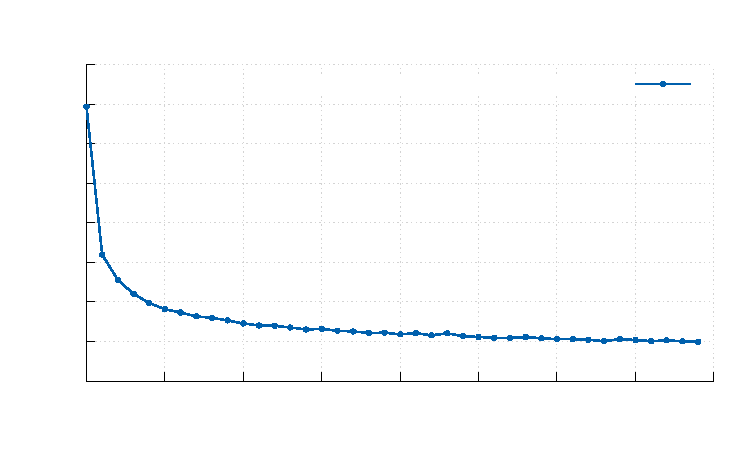
\includegraphics[width={360.00bp},height={216.00bp}]{Figures/solution/training_loss.pdf}}%
    \gplfronttext
  \end{picture}%
\endgroup

	\caption{Graf zobrazuje pozorovanou konvergenci navržené sítě do lokálního optima při použití Sinkhornova algoritmu.}
	\label{fig:RNN_architecture}
\end{figure}

Pro zpřesnění predikcí neuronové sítě v těchto problematických případech zavedli autoři do výsledné účelové funkce třetí část a to tzv. "Total Variation Loss".
Celková variační vzdálenost může být stejně jako cena optimálního přesunu použita pro porovnání dvou pravděpodobnostních měr \(\mu\) a \(\nu\) na stejném měřitelném prostoru \(\mathcal{A}, \mathcal{F})\) \cite{Total_variation}.
Vzdálenost těchto dvou pravděpodobnostních měr je definovaná následujícím vzorcem. (V literatuře se vyskytuje i verze, kdy je tato vzdálenost definovaná, jako dvojnásobek uvedeného vzorce, čímž se dá zbavit \(\frac{1}{2}\).)

\begin{equation}
\delta_{TV}(\mu, \nu) = \sup_{\mathcal{A} \in \mathcal{F}} (\mu(\mathcal{A}) - \nu(\mathcal{A})) = \frac{1}{2}\|\mu - \nu\|_1
\label{eq:total_variation}
\end{equation}

Budou-li \(\mu\) a \(\nu\) zcela disjunktní a nebudou tedy sdílet žádnou "hmotu", bude hodnota takto definované metriky rovna jedné.
Čím více "hmoty" sdílí, 
Při minimalizaci tedy dochází k tomu, že se \(\mu\) a \(\nu\) mnohem více překrývají a jsou-li identické, je hodnota \(\delta_{TV}(\mu, \nu)\) rovna nule.

\begin{equation}
loss_{TV}(z, \hat{z}) = \delta_{TV} \bigg( \frac{z}{\|z\|_1}, \frac{\hat{z}}{\|\hat{z}\|_1} \bigg)
= \frac{1}{2} \bigg\| \frac{z}{\|z\|_1} - \frac{\hat{z}}{\|\hat{z}\|_1} \bigg\|_1
\label{eq:tv_loss}
\end{equation}


Výsledná účelová funkce je, jak již bylo dříve zmíněno, lineární kombinací funkcí "Counting Loss",  "Optimal Transport Loss" a "Total Variation Loss". Parametry \(\lambda_1\) a \(\lambda_2\) slouží k nastavení, jaký vliv budou mít "Optimal Transport Loss" a "Total Variation Loss" ve výsledné účelové funkci.
Aby autoři zajistili, že "Total Variation Loss" a "Optimal Transport Loss" budou mít stejné měřítko, je výsledek "Total Variation Loss" vynásoben počtem lidí v základní pravdě.

\begin{equation}
loss(z, \hat{z}) = loss_{C}(z, \hat{z}) + \lambda_1 loss_{OT}(z, \hat{z}) + \lambda_2 \|z\|_1 loss_{TV}(z, \hat{z})
\label{eq:overall_loss}
\end{equation}



\endinput